This chapter describes \tern, our first \smt system that
addresses the first challenge on building \smt: how to compute highly reusable
schedules for different inputs? The more reusable a schedule is, the fewer
schedules are needed for all inputs. \tern is also built as a \dmt system,
because determinism is especially useful in testing and debugging multithreaded
programs. Building a system that is both \smt and \dmt is challenging, because
as we described in Chapter~\ref{sec:smt-motivation}, the instability problem in
typical \dmt systems destabilizes program behaviors on input perturbations,
defeating the stability benefit brought by \smt. Therefore, this chapter
also describes our solution on addressing this instability problem.

\section{Introduction} \label{sec:tern-overview}

\tern addresses two crucial research challenges. First, how to compute the set
of schedules for processing inputs?  At the bare minimum, a schedule must be
feasible when enforced on an input, so the execution does not get stuck or
deviate from the schedule.  Ideally, the set of schedules should also be small
for reliability.  One possible idea is to pre-compute schedules using static
source code analysis, but the halting problem makes it undecidable to
statically compute schedules guaranteed to work dynamically.  Another
possibility is to compute schedules on the fly while a program is running,
but the computations may be complex and their overhead high.

Second, how to combine \dmt with \smt? Existing \dmt
systems~\cite{dmp:asplos09,coredet:asplos10,kendo:asplos09} constrain a
multithreaded program to always use the same thread schedule for the same input,
greatly increaseing testing confidence and making bug reproduction much more
easier. Unfortunately, these \dmt systems may defeat the input stability
benefit in \smt: when scheduling the threads to process an
input, existing \dmt systems consider only current input and ignore previous
similar inputs.  This stateless design makes schedules over-dependent on inputs,
so that a slight change to inputs may force a program to (ad)venture into a
vastly different, potentially buggy schedule, defeating the key stability
benefit of \smt.  We call this the \emph{instability} problem. This problem is
confirmed by our results (\S\ref{sec:tern-bug-stable}) from an existing \dmt
system~\cite{coredet:asplos10}. In fact, even with the same input, existing \dmt
systems may still force a program into different schedules for minor changes in
the execution environment such as processor type and shared library.  Thus,
developers may no longer be able to reproduce bugs by running their
program on the bug-inducing input, because their machine may differ from
the machine where the bug occurred. \S\ref{sec:dmt-background} will analyze in
details why this instability problem is inherent in existing \dmt systems.

This chapter presents \tern, a schedule-centric, stateful \smt and \dmt system. 
It addresses the aformentioned two research challenges with a new idea called
\emph{schedule memoization} that memoizes past working schedules and reuses them
for future inputs.  Specifically, \tern maintains a cache of past schedules and
the input constraints required to reuse these schedules.  When an input arrives,
\tern checks the input against the memoized constraints for a compatible
schedule.  If it finds one, it simply runs the program while enforcing
this schedule.  Otherwise, it runs the program to memoize a schedule and
the input constraints of this schedule for future reuse. This schedule-centric
approach maps as many as inputs that satisfy the input constraints to each
schedule, greatly reducing the number of schedules required for all inputs, the
central goal of \smt. This stateful approach stabilizes program behaviors
on input perturbations and avoids the instability problem. In sum, \tern's
schedule memoization is the first approach that implements \smt, and the first
approach that combines \smt and \dmt, greatly reducing the number of schedules
on all inputs as well as the number of schdules on each input (down to one)
barring some limitations~\ref{sec:tern-limit}.

\tern's schedule memoization approach has two major benefits on software
reliability. First, by reusing schedules shown to work, \tern can avoid
potential errors in unknown schedules.  This advantage is illustrated in
Figure~\ref{fig:tern-idea}. A real-world analogy to schedule memoization is the
natural tendencies in humans and animals to follow familiar routes to avoid
possible hazards along unknown routes.  Migrant birds, for example, often
migrate along fixed ``flyways."  We thus name our system after the Arctic Tern,
a bird species that migrates the farthest among all
migrants~\cite{artic-tern-wiki}. Second, \tern makes schedules explicit,
providing flexibility in deciding when to memoize certain schedules.  For
instance, \tern allows developers to populate a schedule cache offline, to avoid
the overhead of doing so online.  Moreover, \tern can check for errors (\eg,
races) in schedules and memoize only the correct ones, thus avoiding the buggy
schedules and amortizing the cost of checking for errors.

To make \tern practical, it must handle server programs which frequently
use threads for performance.  These programs present two challenges for
\tern: (1) they often process client inputs (requests) as they arrive, thus
suffering from \emph{input timing nondeterminism}, which existing \dmt systems
do not handle and (2) they may run continuously, making their schedules
effectively infinite and too specific to reuse.

\tern addresses these challenges using a simple idea called
\emph{windowing}.  Our insight is that server programs tend to return to the
same quiescent states. Thus, \tern splits the continuous request stream of a
server into \emph{windows} and lets the server quiesce in between, so that \tern
can memoize and reuse schedules across windows.  Within a window, it admits
requests only at fixed schedule points, reducing timing nondeterminism.

\begin{figure}[t]
\centering
\includegraphics[width=.5\textwidth]{tern/figures/idea.eps}
\caption{\small{\em Advantage of schedule memoization.}  Each solid shape
  represents an input, and each curved line a schedule.  Schedule
  memoization reuses schedules when possible, avoiding bugs in unknown
  schedules and making program behaviors repeatable across similar
  inputs.}
\label{fig:tern-idea}
\end{figure}%% % background on nondeterminism


We implemented \tern in Linux.  It runs as ``parasitic"
user-space schedulers within the application's address space, overseeing
the decisions of the OS scheduler and synchronization library.  It
memoizes and reuses synchronization orders as schedules to increase
performance and reuse rates. It tracks input constraints using
\klee~\cite{klee:osdi08}, a symbolic execution engine.  Our implementation
is software-only, works with general C/C++ programs using \pthread, and
requires no kernel modifications and only a few lines of modification to
applications, thus simplifying deployment.

We evaluated \tern on a diverse set of 14 programs, including two server
programs \apache~\cite{apache} and \mysql~\cite{mysql}, a parallel
compression utility \pbzip~\cite{pbzip2}, and 11 scientific programs in
\splash~\cite{splash2}.  Our workload included a Columbia CS web trace and
benchmarks used by \apache and \mysql developers.  Our results show that

\begin{enumerate}

\item \tern is easy to use.  For most programs, we modified only a few
  lines to adapt them to \tern.

\item \tern enforces stability across different inputs.  In particular, it
  reused 100 schedules to process 90.3\% of a 4-day Columbia CS web trace.
  Moreover, while an existing \dmt system~\cite{coredet:asplos10} made
  three concurrency bugs inconsistently occur or disappear depending on minor
  input changes, \tern's memoized schedules consistently avoided these bugs.

\item \tern has reasonable overhead.  For nine out of fourteen
  evaluated programs, \tern has negligible overhead or improves
  performance; for the other programs, \tern has up to 39.1\%
  overhead.

\item \tern makes threads deterministic.  For twelve out of fourteen
  evaluated programs, the schedules \tern memoized can be deterministically
  reused barring the assumption discussed in \S\ref{sec:tern-impl}.

\end{enumerate}

Our main conceptual contributions are that we addressed the two research
challenges on building a system that is both \smt and \dmt with a new idea
called schedule memoization. To make \tern practically support server programs
that have input timing nondeterminism and infinite schedules, we proposed
another new idea called windowing. Our engineering contributions include the
\tern system and its evaluation on real programs.  To the best of our knowledge,
\tern is the first \smt and \dmt system, the first to mitigate input timing
nondeterminism, and the first shown to work on programs as large, complex, and
nondeterministic as \apache and \mysql.

This chapter is organized as follows.  We first present a background
(\S\ref{sec:tern-background}) and a high-level design of
\tern (\S\ref{sec:tern-design}). We then describe \tern's interface
(\S\ref{sec:tern-annotations}), schedule memoization for batch programs
(\S\ref{sec:tern-batch}), and windowing to extend \tern to server programs
(\S\ref{sec:tern-window}).  We then present refinements we made to optimize
\tern (\S\ref{sec:tern-impl}).  Lastly, we show our experimental results
(\S\ref{sec:tern-evaluation}), discuss related work (\S\ref{sec:tern-related}),
and summarize \tern (\S\ref{sec:tern-summary}).
